\documentclass[aspectratio=169]{beamer}
\usefonttheme{serif}
\usepackage{xeCJK}
\usepackage{fontspec}
\usepackage{graphicx}
\usepackage{listings}
\usepackage{xcolor}
\usepackage{indentfirst}
\usepackage{tikz}
\usepackage{amssymb}
\usepackage{amsthm}
\usepackage{amsmath}
\usepackage{tabularx}
\usepackage{hyperref}
\usepackage{ulem}
\usepackage{version}
\usepackage{thmtools}
\usepackage{qtree}
\usepackage{algpseudocode}
\usepackage{mathtools}
\usepackage{multicol}
\usepackage{xcolor}

\AtBeginDocument{%
    \DeclareSymbolFont{pureletters}{T1}{\mathfamilydefault}{\mddefault}{it}%
    }

\XeTeXlinebreaklocale "zh"
\XeTeXlinebreakskip = 0pt plus 1pt

\setCJKmainfont{NotoSansTC-Medium.otf}
\setmainfont{JetBrainsMono-SemiBold.ttf}
\usetikzlibrary{arrows,decorations.markings,decorations.pathreplacing}
\newenvironment{Hint}{\noindent\textbf{Hint.}}{}

\tikzstyle {graph node} = [circle, draw, minimum width=1cm]
\tikzset{edge/.style = {decoration={markings,mark=at position 1 with %
            {\arrow[scale=2,>=stealth]{>}}},postaction={decorate}}}

\lstset{
    basicstyle=\ttfamily\normalsize,
    numberstyle=\normalsize,
    numbers=left,
    stepnumber=1,
    numbersep=3pt,
    commentstyle=\color{black!50},
    keywordstyle=\color{white!0!blue},
    stringstyle=\color{black!50!green},
    showspaces=false,
    showstringspaces=false,
    showtabs=false,
    tabsize=4,
    captionpos=b,
    breaklines=true,
    breakatwhitespace=false,
    escapeinside={\%*}{*)},
    morekeywords={*}
}

\AtBeginSection[]{
  \begin{frame}
  \vfill
  \centering
  \begin{beamercolorbox}[sep=8pt,center,shadow=true,rounded=true]{title}
    \usebeamerfont{title}\insertsectionhead\par%
  \end{beamercolorbox}
  \vfill
  \end{frame}
}

\title{圖論 III}
\author{Koying}
\date{2022-07-14}

\usetheme{Madrid}
\usecolortheme{default}
\setbeamertemplate{itemize items}[square]
\setbeamertemplate{enumerate items}[default]
\setbeamertemplate{blocks}[default]
\lstdefinestyle{myStyle}{
    belowcaptionskip=1\baselineskip,
    breaklines=true,
    frame=none,
    numbers=none, 
    basicstyle=\footnotesize\ttfamily,
    keywordstyle=\bfseries\color{green!40!black},
    commentstyle=\itshape\color{purple!40!black},
    identifierstyle=\color{blue},
    backgroundcolor=\color{gray!10!white},
}

\begin{document}

    \begin{frame}
        \titlepage
    \end{frame}

    \begin{frame}{目錄}
        \begin{itemize}
            \item 用 RMQ 解 LCA 問題
            \item 時光倒流
            \item 最短路問題
        \end{itemize}
    \end{frame}

    \section{用 RMQ 解 LCA 問題}

    \begin{frame}{用 RMQ 解 LCA 問題}
        \begin{itemize}
            \item<1-> 還記得圖論 II 的 LCA 問題嗎
            \item<2-> 還記得圖論 I 的樹壓平嗎
            \item<3-> 在圖論 I 的樹壓平中,我們只有在出點以及入點的時候才會將該事件加入 ett 陣列中
            \item<3-> 但其實還忽略了一種事件:經過一個點
        \end{itemize}
    \end{frame}

    \begin{frame}{用 RMQ 解 LCA 問題}
        \begin{itemize}
            \item 使用圖論 I 的方式記錄的話,會長這樣:
            \begin{center}
                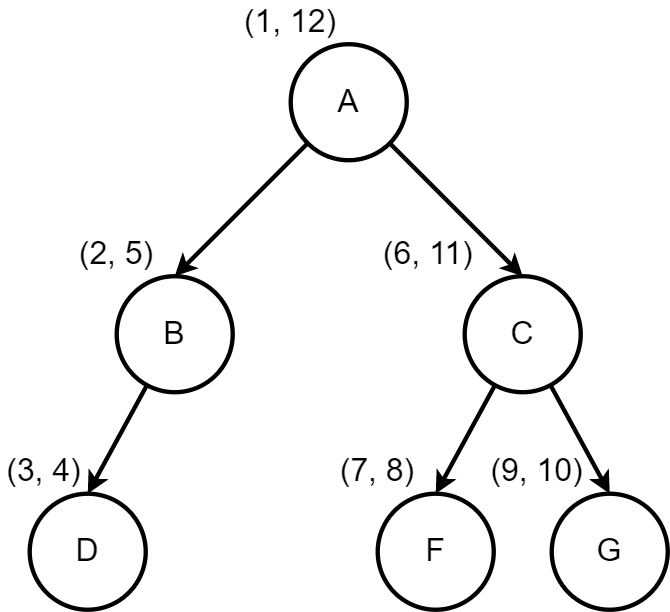
\includegraphics[height=0.7\textheight]{src/ett_1.png}
            \end{center}
        \end{itemize}
    \end{frame}

    \begin{frame}{用 RMQ 解 LCA 問題}
        \begin{itemize}
            \item<1-> 我們會發現從 F 經過 C 到 G 的過程中,C 是沒有被記錄到的
            \item<2-> 這會使得我們只能判斷子孫沒有辦法判斷共同祖先
            \item<3-> 所以我們會將記錄入點、出點改成紀錄更改位置
        \end{itemize}
    \end{frame}

    \begin{frame}{用 RMQ 解 LCA 問題}
        \begin{itemize}
            \item 按照這個方法做就會變成這樣:
            \begin{center}
                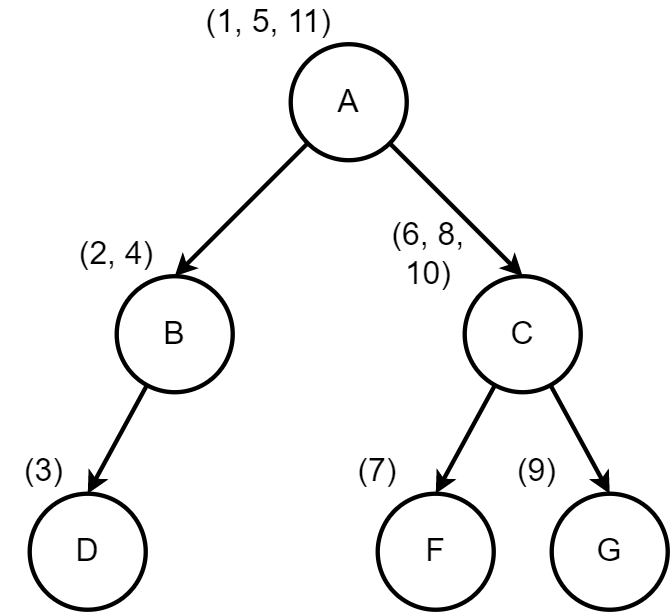
\includegraphics[height=0.7\textheight]{src/ett_2.png}
            \end{center}
        \end{itemize}
    \end{frame}

    \begin{frame}{用 RMQ 解 LCA 問題}
        \begin{itemize}
            \item 如果我們將他寫成一個序列就會長成這樣
            \begin{center}
                \begin{tabular}{c|c|c|c|c|c|c|c|c|c|c|c}
                    ett & 01 & 02 & 03 & 04 & 05 & 06 & 07 & 08 & 09 & 10 & 11\\
                    \hline
                    V & A & B & D & B & A & C & F & C & G & C & A
                \end{tabular}
            \end{center}
        \end{itemize}
    \end{frame}

    \begin{frame}{用 RMQ 解 LCA 問題}
        \begin{itemize}
            \item 除此之外,我們還可以加上深度
            \begin{center}
                \begin{tabular}{c|c|c|c|c|c|c|c|c|c|c|c}
                    ett & 01 & 02 & 03 & 04 & 05 & 06 & 07 & 08 & 09 & 10 & 11\\
                    \hline
                    V & A & B & D & B & A & C & F & C & G & C & A\\
                    \hline
                    dep & 1 & 2 & 3 & 2 & 1 &2 & 3 & 2 & 3 & 2 & 1
                \end{tabular}
            \end{center}
        \end{itemize}
    \end{frame}

    \begin{frame}{用 RMQ 解 LCA 問題}
        \begin{itemize}
            \item<1-> 我們可以發現到:位於一個點 a 的出點以及點 b 的入點之間的所有點之中,深度最小的一個,就是 LCA(a, b)
            \item<2-> 所以我們只需要維護 ett 上的區間最小深度,就可以算出 LCA(a, b)
            \item<3-> 這部分只需要使用資料結構 II 所教的 Sparse Table 就可以了
        \end{itemize}
    \end{frame}

    \begin{frame}{LCA 例題}
        \begin{block}{ZJ d767 血緣關係}
            給一棵樹,求兩點之間的 LCA 以及距離
        \end{block}

        \begin{itemize}
            \item 參考程式:d767.cpp
        \end{itemize}
    \end{frame}

    \section{時光倒流}

    \begin{frame}{時光倒流}
        我們先來看這一題
        \begin{block}{ABC120 D - Decayed Bridges}
            湖上共有 n 個島嶼,m 座橋,第 i 座橋連接第 $a_i, b_i$ 座島嶼\\
            請輸出 m 行,第 i 行代表將編號 $1 \sim i$ 座橋拿掉之後,島嶼會形成幾個連通塊? $n, m \le 10^5$
        \end{block}

        \begin{itemize}
            \item<2-> 乍看之下我們好像會需要一種能夠計算拔邊之後連通塊數量的方法
            \item<3-> 但這樣很麻煩,也不好做
            \item<4-> 如果我們把他反過來看呢?
            \item<5-> 會發現到,拔邊就變成了加邊
        \end{itemize}
    \end{frame}

    \begin{frame}{時光倒流}
        我們先來看這一題
        \begin{block}{ABC120 D - Decayed Bridges}
            湖上共有 n 個島嶼,m 座橋,第 i 座橋連接第 $a_i, b_i$ 座島嶼\\
            請輸出 m 行,第 i 行代表將編號 $1 \sim i$ 座橋拿掉之後,島嶼會形成幾個連通塊? $n, m \le 10^5$
        \end{block}

        \begin{itemize}
            \item<1-> 但我們要怎麼知道加邊之後的連通塊數量呢?
            \item<2-> 不知道大家還記不記得有這麼一個資料結構支援將兩個集合合併
            \item<3-> 沒錯,就是並查集
            \item<4-> 我們只要將題目的意思反著做,並用並查集維護每次加邊之後的連通塊數量,就可以很輕鬆的解出這種題目了
            \item<5-> 這就是經典的\textbf{時光倒流}
        \end{itemize}
    \end{frame}

    \section{最短路問題}

    \begin{frame}{最短路問題的類型}
        \begin{itemize}
            \item<1-> 最短路主要分成兩種類型:
            \item<2-> 單點源最短路問題:求一個固定起點到其他點的最短距離
            \item<2-> 全點對最短路問題:求任意起點跟終點的最短距離
        \end{itemize}
    \end{frame}

    \section{單點源最短路問題}

    \section{0-1 BFS}

    \begin{frame}
        \begin{itemize}
            \item<1-> 今天如果是一張邊權都是 1 的圖,要求起點到某個點的距離
            \item<2-> 那我們就直接做 BFS 就可以了
            \item<3-> 但如果今天邊權是 1 或是 0 呢?
        \end{itemize}
    \end{frame}

    \begin{frame}
        \begin{itemize}
            \item<1-> 回想 BFS 的 queue 會有甚麼特性呢?
            \item<2-> 我們會發現到,越早被 pop 出來的,他的距離就會越短
            \item<3-> 也就是說 BFS 的 queue 裡面會呈現\textbf{單調性}
            \item<4-> 只要能夠滿足 queue 裡面的單調性,我們就能夠利用 BFS 從距離近的點走到距離遠的點的特性來得到最短距離了
        \end{itemize}
    \end{frame}

    \begin{frame}
        \begin{itemize}
            \item<1-> 至於該怎麼維護呢?
            \item<2-> 當邊權是 1 的時候,就跟一般的 BFS 一樣,push 到最後面就可以了
            \item<3-> 但當邊權是 0 的時候,我們 push 到後面就沒有辦法維護單調性
            \item<4-> 那簡單,我們就 push 到前面就好嘛
            \item<4-> 所以,我們將 BFS 的 queue 改成 deque 就可以做 0-1 BFS 了
        \end{itemize}
    \end{frame}

    \begin{frame}{0-1 BFS 例題}
        \begin{block}{CF 173B Chamber of Secrets}
            有一個二維平面由 . 以及 \# 組成,現在有一道雷射光從左上角往右射出\\
            每次遇到 \# 的話可以選擇往四個方向射出,如果有轉方向的話會需要 1 點花費,往原本的方向則不需要花費\\
            求最少需要幾點花費才有辦法使得雷射光到達右下角
        \end{block}

        \begin{itemize}
            \item<2-> 不難發現這其實就是一個權重為 0/1 的圖
            \item<3-> 如果走到 .,那就直接往同方向擴散
            \item<3-> 如果走到的是 \#,那就可以往四個方向擴散
            \item<3-> 參考程式:173B.cpp
        \end{itemize}
    \end{frame}

    \section{Dijkstra 演算法}

    \begin{frame}{鬆弛}
        \begin{itemize}
            \item<1-> 在開始後面的演算法之前,我們需要先知道什麼是鬆弛
            \item<2-> 對於兩個點 u, v,假設由起點到這兩個點的距離分別是 dis(u), dis(v)
            \item<3-> 若存在一條邊從 u 連接到 v,邊權為 w,且 dis(u) + w < dis(v)
            \item<4-> 那麼我們就可以使用這條邊來\textbf{鬆弛}dis(v),讓 dis(v) = dis(u) + w
        \end{itemize}
    \end{frame}

    \begin{frame}{Dijkstra}
        \begin{itemize}
            \item<1-> 前面提到說,我們在做 BFS 的時候,需要維護 queue 裡面的距離需要呈現單調性
            \item<2-> 當邊權為 0/1 時我們會用 deque 來維護單調性
            \item<3-> 那如果是任意正整數呢?
            \item<4-> 簡單,就改成 priority\_queue 來維護單調性就好啦
            \item<5-> 好,你會 Dijkstra 演算法了!
        \end{itemize}
    \end{frame}

    \begin{frame}{Dijkstra}
        \begin{itemize}
            \item<1-> 在實作上,我們會使用一個陣列 dis 紀錄起點到每個點的距離
            \item<2-> 起初先將所有 dis[i] 設為 $\infty$,並將 dis[s] 設為 0 (s 為起點)
            \item<3-> 接著我們會開一個優先取出最小值的 priority\_queue<pair<int, int>> pq,first 代表距離,second 代表點的編號
            \item<4-> 接著在每次取出 pq.top() 時檢查與其相鄰的所有點是否有可能被鬆弛,要是被鬆弛,那就將該點丟入 pq 內
            \item<5-> 需要注意的是,如果某個點已經被其他邊鬆弛過了,也就是 pq 內的距離並不是最小的,那就直接忽略這筆資料
            \item<6-> Dijkstra 只適用在非負權圖上,如果有出現負權,那麼不保證出來的答案會是對的
            \item<7-> 每一條邊最多只會被放進 pq 裡一次,所以時間複雜度 $\mathcal{O}(\lvert E \rvert log \lvert E \rvert)$
        \end{itemize}
    \end{frame}

    \begin{frame}{Dijkstra}
        \begin{itemize}
            \item 假設我們有這樣一張圖:
            \begin{center}
                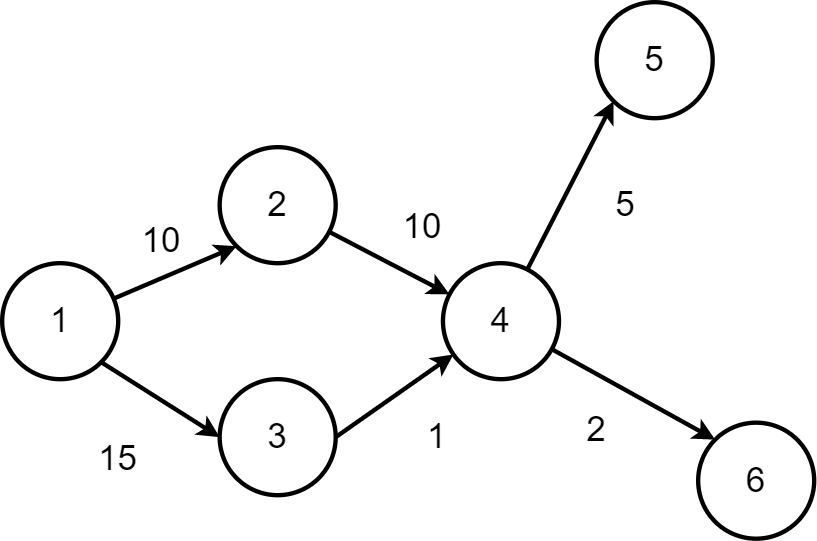
\includegraphics[width=0.4\textwidth]{src/dijkstra_1.png}
            \end{center}
        \end{itemize}

        \begin{center}
            \begin{tabular}{c|c|c|c|c|c|c}
                V & 1 & 2 & 3 & 4 & 5 & 6 \\
                \hline
                dis & 0 & $\infty$ & $\infty$ & $\infty$ & $\infty$ & $\infty$
            \end{tabular}
        \end{center}
    \end{frame}

    \begin{frame}{Dijkstra}
        \begin{itemize}
            \item 首先我們會先使用這條邊來鬆弛點 2
            \begin{center}
                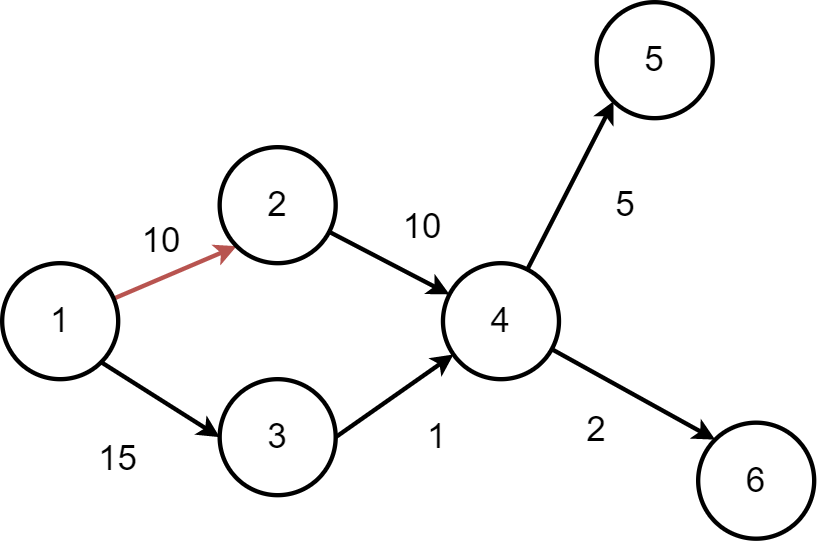
\includegraphics[width=0.4\textwidth]{src/dijkstra_2.png}
            \end{center}
        \end{itemize}

        \begin{center}
            \begin{tabular}{c|c|c|c|c|c|c}
                V & 1 & 2 & 3 & 4 & 5 & 6 \\
                \hline
                dis & 0 & 10 & $\infty$ & $\infty$ & $\infty$ & $\infty$
            \end{tabular}
        \end{center}
    \end{frame}

    \begin{frame}{Dijkstra}
        \begin{itemize}
            \item 接著鬆弛點 3:
            \begin{center}
                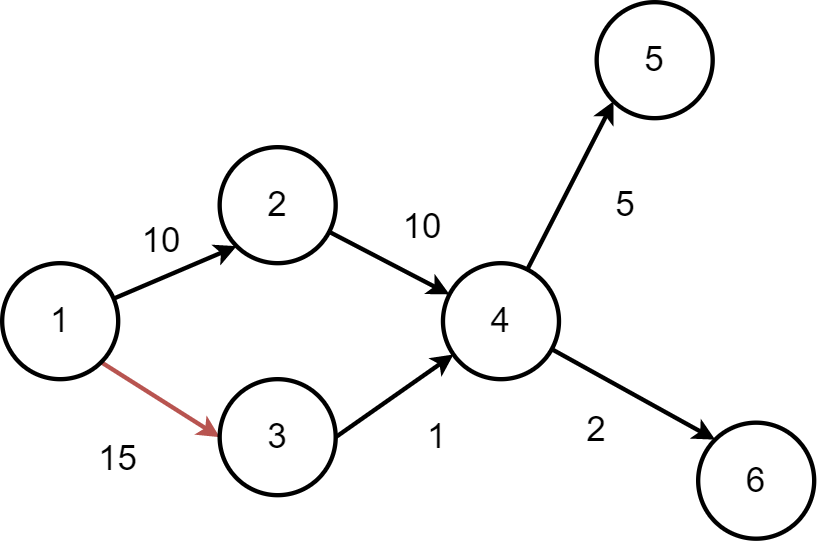
\includegraphics[width=0.4\textwidth]{src/dijkstra_3.png}
            \end{center}
        \end{itemize}

        \begin{center}
            \begin{tabular}{c|c|c|c|c|c|c}
                V & 1 & 2 & 3 & 4 & 5 & 6 \\
                \hline
                dis & 0 & 10 & 15 & $\infty$ & $\infty$ & $\infty$
            \end{tabular}
        \end{center}
    \end{frame}

    \begin{frame}{Dijkstra}
        \begin{itemize}
            \item 然後是點 4:
            \begin{center}
                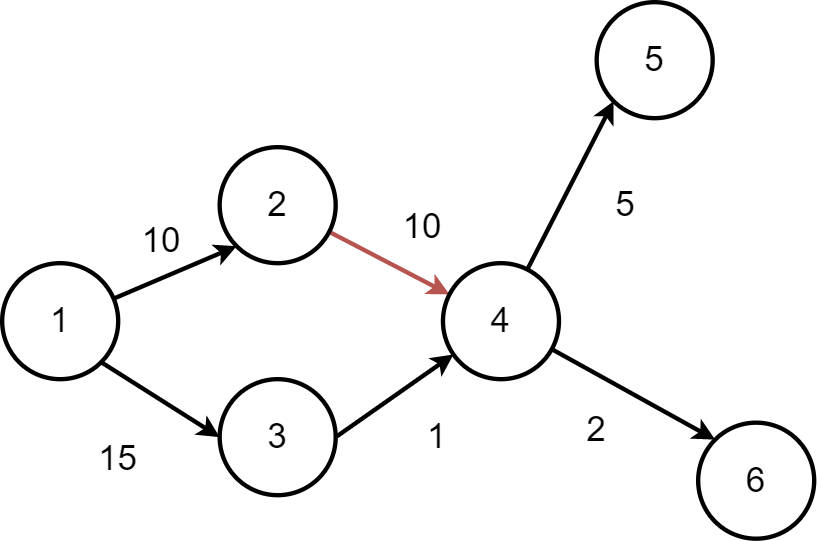
\includegraphics[width=0.4\textwidth]{src/dijkstra_4.png}
            \end{center}
        \end{itemize}

        \begin{center}
            \begin{tabular}{c|c|c|c|c|c|c}
                V & 1 & 2 & 3 & 4 & 5 & 6 \\
                \hline
                dis & 0 & 10 & 15 & 20 & $\infty$ & $\infty$
            \end{tabular}
        \end{center}
    \end{frame}

    \begin{frame}{Dijkstra}
        \begin{itemize}
            \item 然後我們發現點 4 還可以被鬆弛:
            \begin{center}
                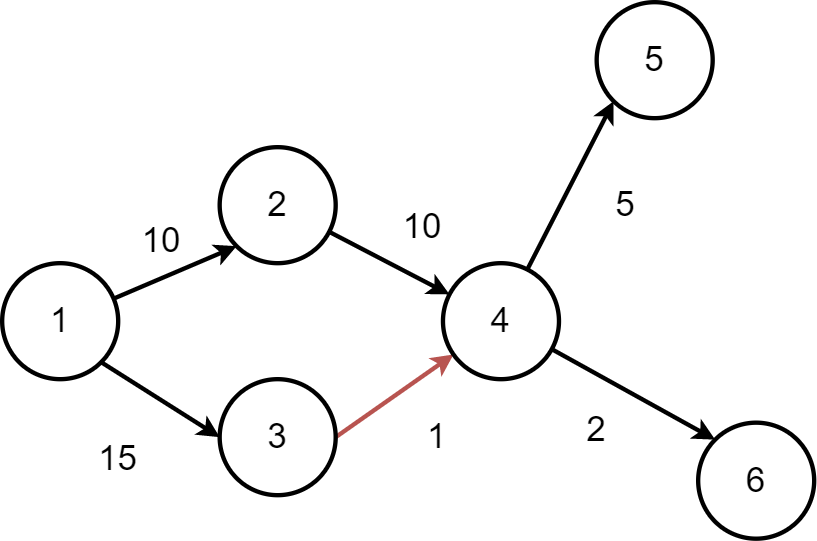
\includegraphics[width=0.4\textwidth]{src/dijkstra_5.png}
            \end{center}
        \end{itemize}

        \begin{center}
            \begin{tabular}{c|c|c|c|c|c|c}
                V & 1 & 2 & 3 & 4 & 5 & 6 \\
                \hline
                dis & 0 & 10 & 15 & 16 & $\infty$ & $\infty$
            \end{tabular}
        \end{center}
    \end{frame}

    \begin{frame}{Dijkstra}
        \begin{itemize}
            \item 最後將其他的點都鬆弛完畢:
            \begin{center}
                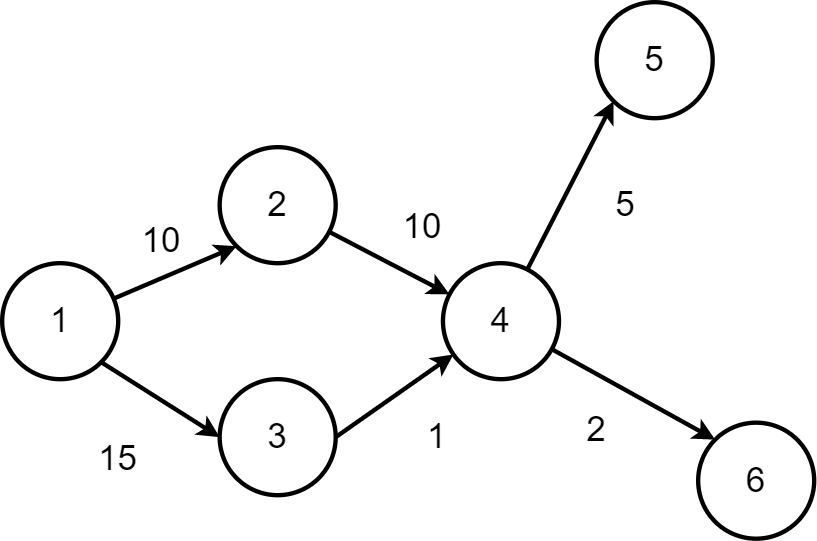
\includegraphics[width=0.4\textwidth]{src/dijkstra_1.png}
            \end{center}
        \end{itemize}

        \begin{center}
            \begin{tabular}{c|c|c|c|c|c|c}
                V & 1 & 2 & 3 & 4 & 5 & 6 \\
                \hline
                dis & 0 & 10 & 15 & 16 & 21 & 18
            \end{tabular}
        \end{center}
    \end{frame}

    \begin{frame}{Dijkstra 例題}
        \begin{block}{CSES 1671 Shortest Routes I}
            求出從起點到其他所有點的最短距離 \\
            $(n \le 10^5, m \le 2 \times 10^5)$
        \end{block}

        \begin{itemize}
            \item 參考程式:Shortest\_Routes\_I.cpp
        \end{itemize}
    \end{frame}
        
    \begin{frame}{Dijkstra 例題}
        \begin{block}{CSES 1012 Investigation}
            給一張圖,求從 1 走到 n 的以下四種數據:
            \begin{enumerate}
                \item 最短路徑
                \item 有幾種最短路徑
                \item 最短路徑最少需要經過幾條邊
                \item 最短路徑最多需要經過幾條邊
            \end{enumerate}
        \end{block}

        \begin{itemize}
            \item<2-> 以下會使用 四種陣列來儲存題目要的四種數據
            \begin{enumerate}
                \item dis[i]:走到點 i 的最短路徑
                \item cnt[i]:走到點 i 有幾種最短路徑
                \item minf[i]:走到點 i 最短路徑最少需要經過幾條邊
                \item maxf[i]:走到點 i 最短路徑最多需要經過幾條邊
            \end{enumerate}
        \end{itemize}
    \end{frame}

    \begin{frame}{Dijkstra 例題}
        \begin{block}{CSES 1012 Investigation}
            給一張圖,求從 1 走到 n 的以下四種數據:
            \begin{enumerate}
                \item 最短路徑
                \item 有幾種最短路徑
                \item 最短路徑最少需要經過幾條邊
                \item 最短路徑最多需要經過幾條邊
            \end{enumerate}
        \end{block}

        \begin{itemize}
            \item<1-> 首先求最短路徑應該沒有問題
            \item<2-> 那該如何求最短路徑有幾種呢?
            \item<3-> 想像我們在用點 u 鬆弛 點 v 時,有三種情況:
            \begin{enumerate}
                \item 可以鬆弛 (dis(u) + e < dis(v))
                \item 剛好一樣 (dis(u) + e = dis(v))
                \item 無法鬆弛(dis(u) + e > dis(v))
            \end{enumerate}
        \end{itemize}
    \end{frame}

    \begin{frame}{Dijkstra 例題}
        \begin{block}{CSES 1012 Investigation}
            給一張圖,求從 1 走到 n 的以下四種數據:
            \begin{enumerate}
                \item 最短路徑
                \item 有幾種最短路徑
                \item 最短路徑最少需要經過幾條邊
                \item 最短路徑最多需要經過幾條邊
            \end{enumerate}
        \end{block}

        \begin{itemize}
            \item<1-> 不難發現到,在無法鬆弛的情況下,cnt[v] 並不會有變化
            \item<2-> 那麼我們就著重在可以鬆弛以及剛好一樣的情況
        \end{itemize}
    \end{frame}

    \begin{frame}{Dijkstra 例題}
        \begin{block}{CSES 1012 Investigation}
            給一張圖,求從 1 走到 n 的以下四種數據:
            \begin{enumerate}
                \item 最短路徑
                \item 有幾種最短路徑
                \item 最短路徑最少需要經過幾條邊
                \item 最短路徑最多需要經過幾條邊
            \end{enumerate}
        \end{block}

        \begin{itemize}
            \item<1-> 可以鬆弛情況代表目前這條路徑取代了原先走到 v 的最短路徑,所以我們會將 cnt[v] 設為 cnt[u]
            \item<2-> 至於剛好一樣的情況,代表要走原本的或是走目前的邊都可以,所以 cnt[v] 就是 cnt[u] + cnt[v]
            \item<3-> 那我們就可以成功的寫出 cnt 的計算方法了
        \end{itemize}
    \end{frame}

    \begin{frame}{Dijkstra 例題}
        \begin{block}{CSES 1012 Investigation}
            給一張圖,求從 1 走到 n 的以下四種數據:
            \begin{enumerate}
                \item 最短路徑
                \item 有幾種最短路徑
                \item 最短路徑最少需要經過幾條邊
                \item 最短路徑最多需要經過幾條邊
            \end{enumerate}
        \end{block}

        \begin{itemize}
            \item<1-> 接著是 minf 以及 maxf 的計算,兩者只是取最大最小的差別
            \item<2-> 一樣,不能鬆弛就不要理他
        \end{itemize}
    \end{frame}

    \begin{frame}{Dijkstra 例題}
        \begin{block}{CSES 1012 Investigation}
            給一張圖,求從 1 走到 n 的以下四種數據:
            \begin{enumerate}
                \item 最短路徑
                \item 有幾種最短路徑
                \item 最短路徑最少需要經過幾條邊
                \item 最短路徑最多需要經過幾條邊
            \end{enumerate}
        \end{block}

        \begin{itemize}
            \item<1-> 可以鬆弛就代表取代,所以 minf[v] = minf[u] + 1,maxf 以此類推
            \item<2-> 剛好一樣的話代表都可以,所以我們就取最優解,minf[v] = min(minf[u], minf[v]),maxf 以此類推
            \item<3-> 如此一來我們就可以算出這一題了
            \item<3-> 參考程式:Investigation.cpp
        \end{itemize}
    \end{frame}

    \begin{frame}{Dijkstra 例題}
        \begin{block}{ABC 252E Road Reduction}
            給一張 n 座城市的國家,計畫興建 m 條雙向道路,每條道路都有他的長度,但是國家預算有限,所以總統希望只興建 n - 1 條道路\\
            請問需要興建哪幾條道路才能讓每座城市之間都互相連通,且第一座城市到其他每一座城市的最小距離和最小 ($n \le 2 \times 10^5$)
        \end{block}

        \begin{itemize}
            \item<1-> 首先我們要知道題目要的其實就是一個生成樹使得第一座城市到其他每一座城市的最小距離和最小
            \item<2-> 那我們要怎麼求出這個生成樹呢?
            \item<3-> 其實不難發現,跑完 dijkstra 之後,有用到的邊其實就是一個生成樹
            \item<4-> 可以簡單的證明一下,假設從點 u 走到點 v 的路徑形成了一個環,那麼從點 u 走到點 v 就會有兩條路徑
            \item<5-> 而兩條路徑中一定有一條是最好的,所以會跟 dijkstra 所做的事矛盾
        \end{itemize}
    \end{frame}

    \begin{frame}{Dijkstra 例題}
        \begin{block}{ABC 252E Road Reduction}
            給一張 n 座城市的國家,計畫興建 m 條雙向道路,每條道路都有他的長度,但是國家預算有限,所以總統希望只興建 n - 1 條道路\\
            請問需要興建哪幾條道路才能讓每座城市之間都互相連通,且第一座城市到其他每一座城市的最小距離和最小 ($n \le 2 \times 10^5$)
        \end{block}

        \begin{itemize}
            \item<1-> 至於題目所求的距離和最短,其實就是將到每個點的最短距離加起來
            \item<2-> 所以我們需要做的就只有把 dijkstra 會需要用到的邊記錄下來,最後直接輸出即可
            \item<3-> 我們可以用一個陣列 from[] 代表在鬆弛時一併紀錄每個點從哪個點鬆弛來的
            \item<4-> 最後再將 from[2] $\sim$ from[n] 輸出出來即可
            \item<4-> 參考程式:ABC252E.cpp
        \end{itemize}
    \end{frame}

    \begin{frame}{Dijkstra 例題}
        \begin{block}{CSES 1195 Flight Discount}
            有 n 座城市,m 條單向航線,你可以選擇在路徑上的某一個航線使用半價券\\
            請問從第 1 個城市飛到第 n 個城市的最小花費 $(n \le 10^5, m \le 2 \times 10^5)$
        \end{block}

        \begin{itemize}
            \item<2-> 會發現在這題中,每個點有兩個狀態:用過折價券以及沒用過折價券,計為 $u_0, u_1$
            \item<3-> 那我們或許可以在建圖的時候將三種可能都建出來:
            \begin{enumerate}
                \item $u_0 \rightarrow v_0$
                \item $u_0 \rightarrow v_1$
                \item $u_1 \rightarrow v_1$
            \end{enumerate}
            \item<4-> 而這就是經典的技巧:建虛點,將不同狀態的點都建出來,以利後面的操作
            \item<5-> 但是這樣會讓我們的邊數直接變成三倍,有沒有比較好的方法呢?    
        \end{itemize}                   
    \end{frame}

    \begin{frame}{Dijkstra 例題}
        \begin{block}{CSES 1195 Flight Discount}
            有 n 座城市,m 條單向航線,你可以選擇在路徑上的某一個航線使用半價券\\
            請問從第 1 個城市飛到第 n 個城市的最小花費 $(n \le 10^5, m \le 2 \times 10^5)$
        \end{block}

        \begin{itemize}
            \item<1-> 我們或許可以不要真的將不同狀態的點都建出來
            \item<2-> 同樣的事情,我們可以直接在做 dijkstra 時直接內建在 pq 的狀態裡就好
            \item<3-> 如此一來就可以省去不少空間
            \item<4-> 雖然建虛點的方式已經夠好了,但是在某些情況下,建虛點會使得你得到 MLE,這時候優化他就很重要了
            \item<4-> 參考程式:Flight\_Discount.cpp
        \end{itemize}
    \end{frame}

    \begin{frame}{Dijkstra 例題}
        \begin{block}{TPR17 pG 高乘載管制}
            有 n 座城市,m 條單向道路,第 i 條道路連接 $a_i, b_i$,過路費 $w_i$\\
            你有 k 張折價券,每張折價券可以讓你在路上的某一條道路上的過路費減半,可以在同一條道路上重複使用\\
            求從 x 走到 y 的最短路徑 $(n \le 2 \times 4, m \le 10^5)$
        \end{block}

        \begin{itemize}
            \item<2-> 看起來似乎跟剛剛的 Flight Discount 頗像的,能不能建虛點呢?
            \item<3-> 可以,但只能拿到 62 分
            \item<4-> 那如果套用剛剛的優化呢?
            \item<5-> 也可以,但是只可以拿到 87 分,不能再高了
        \end{itemize}
    \end{frame}

    \begin{frame}{Dijkstra 例題}
        \begin{block}{TPR17 pG 高乘載管制}
            有 n 座城市,m 條單向道路,第 i 條道路連接 $a_i, b_i$,過路費 $w_i$\\
            你有 k 張折價券,每張折價券可以讓你在路上的某一條道路上的過路費減半,可以在同一條道路上重複使用\\
            求從 x 走到 y 的最短路徑 $(n \le 2 \times 4, m \le 10^5)$
        \end{block}

        \begin{itemize}
            \item<1-> 或許我們可以把使用不同次折價券的狀態分開來做
            \item<2-> 做 k + 1 次 Dijkstra,第 i 次代表使用 i - 1 次折價券的情況
            \item<3-> 假設有兩個點 u, v,中間有一條權重 w 的邊連接,使用了 i 次折價券的最小花費是 dp[i][u]、dp[i][v]
            \item<4-> 那麼我們可以得到一個轉移式:$dp[i][v] = min(dp[i][v], dp[j][v] + \frac{w}{2 ^ (i-j)}) (j < i)$
            \item<5-> 那麼我們就可以在 $\mathcal{O}(k (m (k + \log m)))$ 的時間做出這一題了
        \end{itemize}
    \end{frame}


    \section{Bellman-Ford}

    \begin{frame}{Bellman-Ford}
        \begin{itemize}
            \item<1-> 如果今天邊權可能會是任意正整數,那我們就沒有辦法使用 deque 來維護了
            \item<2-> 我們可以考慮一下剛剛講到的鬆弛
            \item<3-> 考慮一張圖,如果我們走過一次所有的邊並嘗試將端點鬆弛,可以發現只要是深度為 1 的點,都會被鬆弛到
            \item<4-> 如果我們走兩次,那就是深度 $1 \sim 2$ 的點都會被鬆弛到
            \item<5-> 所以我們只要走足夠多次,就可以鬆弛所有的點,得到起點到終點的最短路徑了
        \end{itemize}
    \end{frame}

    \begin{frame}{Bellman-Ford}
        \begin{itemize}
            \item<1-> 那我們要怎麼知道我們要走多少次呢?
            \item<2-> 既然走 x 次就可以鬆弛深度 $1 \sim x$ 的點,那麼一張深度度為 D 的圖就只需要走 D 次就好
            \item<3-> 已知一張圖的最大深度是 |V|,所以我們最終就只需要走 |V| 次就可以了
            \item<4-> 所以 Bellman-Ford 演算法的複雜度就是 $\mathcal{O}(\lvert V \rvert \times \lvert \mid E \rvert)$
            \item<5-> 參考程式:Bellman-Ford.cpp (這段程式碼是 AI 寫的,輸光)
        \end{itemize}
    \end{frame}

    \begin{frame}{SPFA}
        \begin{itemize}
            \item<1-> 但仔細分析之後我們會發現,當跑道很後面時,真正有鬆弛到的點可能非常的少,大多數的點都已經沒有辦法再鬆弛了
            \item<2-> 有沒有辦法省略掉這些無用的步驟呢?
            \item<3-> 我們可以發現到:當一個點 u 被鬆弛,那麼與其相鄰的點 v 才有可能被鬆弛
            \item<4-> 所以我們可以使用一個 queue 維護與哪些點相鄰的有可能被鬆弛,每次都直接從 queue 中找與其相鄰的點來鬆弛即可
            \item<5-> 但是如果出題者有刻意卡的話,是有辦法讓 SPFA 退化到 Bellman-Ford 的 $\mathcal{O}(nm)$ 的,所以 SPFA 通常不會讓你的 Bellman-Ford 變成 AC
        \end{itemize}
    \end{frame}

    \begin{frame}{判斷負環}
        \begin{itemize}
            \item<1-> 當題目不保證邊都是正的時候,有可能會因此出現負環
            \item<2-> 此時在環上的點,如果沒有額外處理的話,很可能就會無限鬆弛
            \item<3-> 所以當我們在做 SPFA 優化時,可以記錄每個點被鬆弛了幾次,若 $> \lvert V \rvert$,那就代表有負環
            \item<4-> 至於 Bellman-Ford 也是同理,如果鬆弛到第 n + 1 輪還可以鬆弛,那就代表有負環
            \item<5-> 因此 Bellman-Ford 以及 SPFA 是可以用在有可能會有負環的圖上的
        \end{itemize}
    \end{frame}

    \begin{frame}{Bellman-Ford 例題}
        \begin{block}{CSES 1673 High Score}
            共有 n 個房間,m 條道路,第 i 條道路連接房間 a, b,經過他會得到 c 點分數,分數有正有負\\
            求從房間 1 走到房間 n 的最高分數 $(n \le 2500, m \le 5000)$
        \end{block}

        \begin{itemize}
            \item<2-> 首先我們轉換一下問題,求 1 $\sim$ n 的最高分數,其實就是將所有的道路都改成負的,然後再求最短路徑
            \item<3-> 因為分數有正有負,所以我們不能直接使用 dijkstra 來做
            \item<4-> 先做一次 Bellman-Ford,如果沒有負環,那麼最終的結果就是最高分數
            \item<5-> 那如果有呢?
        \end{itemize}
    \end{frame}

    \begin{frame}{Bellman-Ford 例題}
        \begin{block}{CSES 1673 High Score}
            共有 n 個房間,m 條道路,第 i 條道路連接房間 a, b,經過他會得到 c 點分數,分數有正有負\\
            求從房間 1 走到房間 n 的最高分數 $(n \le 2500, m \le 5000)$
        \end{block}

        \begin{itemize}
            \item<1-> 先思考一個問題:有負環是否代表最高分數就會無限大?
            \item<2-> 答案是否的,即使他有負環,但如果不在從 1 走到 n 的道路上,那依舊不會影響到最高分數
            \item<3-> 所以說,如果圖中有一個負環,需要使得這個環與點 1 還有點 n 連通,才會使得分數變無限大
            \item<4-> 因為 n 很小,所以我們可以枚舉每個點當作起點,判斷是否有環出現,$\mathcal{O}(nm)$
            \item<5-> 判斷環的部分圖論 I 有講過了,至於判斷負環只需要在判斷條件上加一個權和為負的條件即可
        \end{itemize}
    \end{frame}

    \begin{frame}{Bellman-Ford 例題}
        \begin{block}{CSES 1673 High Score}
            共有 n 個房間,m 條道路,第 i 條道路連接房間 a, b,經過他會得到 c 點分數,分數有正有負\\
            求從房間 1 走到房間 n 的最高分數 $(n \le 2500, m \le 5000)$
        \end{block}

        \begin{itemize}
            \item<1-> 至於怎麼判斷跟 1、n 是否連通呢?
            \item<2-> 簡單!dfs 一下就好嘛
            \item<3-> 最後,如果沒有找到一個會影響答案的環,那我們就做一次 Bellman-Ford,得出最後的答案
            \item<4-> 此外,這題有一個實作重點是:邊需要按照權重大小排序,如此一來在 dfs 找負環時,才會優先找權重最小的
            \item<4-> 參考程式:High\_Score.cpp
        \end{itemize}
    \end{frame}

    \section{差分約束}

    \begin{frame}{差分約束}
        \begin{block}{差分約束}
            假設有 n 個變數,m 個約束條件,一個約束條件有可能是下列兩種情況:
            \begin{itemize}
                \item $a_i - b_i \le c_i$
                \item $a_i - b_i \ge c_i$
            \end{itemize}
            求是否有一組解能滿足所有約束條件
        \end{block}

        \begin{itemize}
            \item<2-> 我們轉換一下第一個式子,會發現可以轉成 $a_i - c_i \le b_i$
            \item<3-> 這其實就是鬆弛的條件,當 $b_i < a_i - c_i$ 時,就把 $b_i$ 鬆弛為 $a_i - c_i$
            \item<4-> 雖然跟最短路的鬆弛條件不一樣,但是做的事是差不多的
            \item<5-> 所以對於這種狀況,我們只需要連一條邊 $a_i \rightarrow b_i$,權重為 $-c_i$ 就可以了
            \item<6-> 至於第二條式子,轉換之後就會是連一條邊 $b_i \rightarrow a_i$,權重為 $c_i$
        \end{itemize}
    \end{frame}    

    
    \begin{frame}{差分約束}
        \begin{block}{差分約束}
            假設有 n 個變數,m 個約束條件,一個約束條件有可能是下列兩種情況:
            \begin{itemize}
                \item $a_i - b_i \le c_i$
                \item $a_i - b_i \ge c_i$
            \end{itemize}
            求是否有一組解能滿足所有約束條件
        \end{block}

        \begin{itemize}
            \item<1-> 建完圖之後,我們只要對他做最短路徑,就可以求出解了
            \item<2-> 若圖中出現負環,那就代表無解
            \item<2-> 參考程式:Difference\_Constraints.cpp
        \end{itemize}
    \end{frame}    

    \begin{frame}{差分約束例題}
        \begin{block}{2011-2012 Stanford Local Contest, 8 October, 2011 G Guessing Game}
            有兩個數列 a, b,a 的長度為 n, b 的長度為 m,共有 q 個約束條件,一個約束條件有可能是下列兩種情況:
            \begin{itemize}
                \item $a_i + b_i \le c_i$
                \item $a_i + b_i \ge c_i$
            \end{itemize}
            求是否有可能出現一組解
        \end{block}

        \begin{itemize}
            \item<2-> 該怎麼將 $a + b \le c$ 轉換成 $a - b \le c$ 呢?
            \item<3-> 會發現到跟原本式子的差別就是 b 變成 -b 了
            \item<4-> 那簡單,我們都先把 b 變成 -b 就可以吧 a + b 換成 a - b 了
            \item<5-> 成功轉換之後就可以直接做了
            \item<5-> 參考程式:10015G.cpp
        \end{itemize}
    \end{frame}

    \section{全點對最短路徑}

    \section{n 次 Dijkstra}

    \begin{frame}{n 次 Dijkstra}
        \begin{itemize}
            \item 如果要在一個非負權圖上求全點對最短路徑,那簡單,我們就枚舉每個點為起點,做 n 次 Dijkstra 就好了嘛
            \item 時間複雜度:$\mathcal{O}(\lvert V \rvert\lvert E \rvert log \lvert E \rvert)$
        \end{itemize}
    \end{frame}

    \section{Floyd-Warshall 演算法}

    \begin{frame}{Floyd-Warshall}
        \begin{itemize}
            \item<1-> 對於一個點 a 到一個點 b 的最短路徑,假設中間經過一個點 c,已知 a $\rightarrow$ c 的最短路徑 dis(a, c) 以及 c $\rightarrow$ b 的最短路徑 dis(c, b)
            \item<2-> 那麼要怎麼求得 a 經過 c 走到 b 的最短路徑呢?
            \item<3-> 可以發現答案就是 dis(a, c) + dis(c, b)
        \end{itemize}
    \end{frame}

    \begin{frame}{Floyd-Warshall}
        \begin{itemize}
            \item<1-> 那拿出我們塵封已久的 DP,就可以設計出一個狀態:dp[k][i][j] 代表 i 到 j 經過前 k 個點的最短路徑
            \item<2-> 那麼我們就可以得到一個轉移式:dp[k][i][j] = min(dp[k - 1][i][j], dp[k - 1][i][k] + dp[k - 1][k][j])
            \item<3-> 然後你會發現,dp[k] 只跟 dp[k - 1] 有關係,所以我們可以滾動成 $2 \times n \times n$ 的狀態
            \item<4-> 但你再仔細看一次,會發現 dp[k][i][j] 本來就是 dp[k - 1][i][j] 了,然後 dp[k - 1][i][k] 也跟 dp[k][i][k] 沒什麼兩樣,所以我們其實可以直接省略掉第一維
            \item<5-> 那麼就可以得到最終的轉移式:dp[i][j] = min(dp[i][j], dp[i][k] + dp[k][j])
            \item<5-> 時間複雜度:$\mathcal{O}(n^3)$
        \end{itemize}
    \end{frame}

    \begin{frame}{Floyd-Warshall 例題}
        \begin{block}{CSES 1672 Shortest Routes II}
            給一張圖,對於每筆詢問輸入點 a, b,請輸出 a 到 b 的最短路徑 $(n \le 500, m \le n^2)$
        \end{block}

        \begin{itemize}
            \item<2-> 注意到這個題目有可能是個稠密圖,在 m 接近 $n^2$ 時如果使用 n 次 Dijkstra 的話,複雜度會是 $\mathcal{O}(n^3 \log n^2)$
            \item<3-> 這個複雜度是比 Floyd-Warshall 的 $\mathcal{O}(n^3)$ 還要慢的
            \item<4-> 因此在稠密圖上我們一般都會使用 Floyd-Warshall
            \item<4-> 參考程式:Shortest\_Routes\_II.cpp
        \end{itemize}
    \end{frame}

    \begin{frame}{Floyd-Warshall 例題}
        \begin{block}{ABC 208D Shortest Path Queries 2}
            有一張有向圖,請求出 $\displaystyle\sum_{s=1}^{N}\sum_{t=1}^{N}\sum_{k=1}^{N} f(s, t, k)$\\
            $f(s, t, k)$ 代表從 s 走到 t,只經過前 k 個點的最短距離,若無法經由前 k 個點從 s 走到 t,則 $f(s, t, k) = 0$
        \end{block}

        \begin{itemize}
            \item<2-> 仔細一看會發現,這就是求 Floyd-Warshall 每個狀態點的和嘛
            \item<3-> 所以我們只要一邊做 Floyd-Warshall,一邊把每個狀態的最短路徑記錄下來就好
            \item<4-> 需要額外判斷到不了的情況
            \item<4-> 參考程式:ABC208D.cpp
        \end{itemize}
    \end{frame}

    \begin{frame}{Floyd-Warshall 例題}
        \begin{block}{ABC 243E Edge Deletion}
            有一個帶權無向圖,請問你最多可以刪除幾條邊,使剩下的邊滿足以下兩點:
            \begin{enumerate}
                \item 圖連通
                \item 對於任意的 (s, t),從 s 走到 t 的最短路徑與不刪除時相同
            \end{enumerate}
        \end{block}

        \begin{itemize}
            \item<2-> 這題跟前面 Dijkstra 那題有點類似,都是在求哪些邊是必要的,哪些不是
            \item<3-> 對於一條連接 a, b,權重為 c 的邊,若有另外一條從 a 經過其他點到 b 的道路 $\le c$,那麼就代表這條邊不是必要的
            \item<4-> 只要在 Floyd-Warshall 完檢查有幾條邊滿足以上的條件,就可以算出答案了
            \item<4-> 參考程式:ABC243E.cpp
        \end{itemize}
    \end{frame}
\end{document}